\subsection{Data Collection}
We obtained hourly closing price data for BTC-USD and ETH-USD from December 1, 2023, to December 1, 2024, using the yfinance API.

\subsection{HAR Modeling}
\label{sec:return_normolize}

% \subsubsection{Mathematical Formulations for GARCH}
% We present the mathematical formulations for GARCH, EGARCH, GJR-GARCH, and others, explaining how each model captures volatility and asymmetry.

\subsubsection{Building HAR and GARCH Predictions}
The HAR model uses daily, weekly, and monthly realized volatility values to predict the next value, as in Formula~\ref{har-formula}.

As GARCH modeling was the focus of our previous research, we will not delve into the details and only mention that the GARCH(p, q) model directly predicts the current volatility, represented as follows:

\begin{equation}
    \widehat{\text{RV}}_t^2 = \omega + \sum_{i=1}^{q} \alpha_i u_{t-1}^2 + \sum_{j=1}^{p} \beta_j \tilde{\sigma}_{t-j}^2
\end{equation}

Here, \(\tilde{\sigma}_t^2\) denotes the conditional volatility at time \(t\).

To prevent data leaks, the final prediction of the model was obtained using the expanding window method: the model was fitted on data from the moment \(t=0\) to \(t-1\) and then made an estimation \(\widehat{\text{RV}}_t\). The result of this process is shown in Figure~\ref{fig:predictions}.

\begin{figure}[ht]
    \centering
    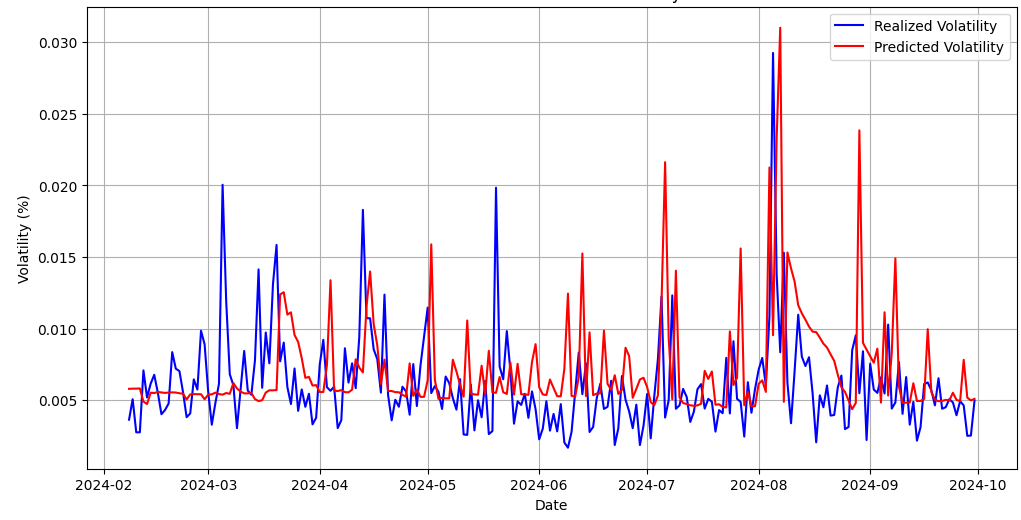
\includegraphics[width=0.8\textwidth]{img/realized_vs_pred.png}  % Adjust width to fit the page
    \caption{Results of HAR Predictions}
    \label{fig:predictions}
\end{figure}

\subsection{Evaluation}
To estimate model performance, we computed the Mean Squared Error (MSE) and Mean Absolute Error (MAE) between the realized volatility values \(\text{RV}_t\) (i.e., ground truth) and GARCH predictions \(\widehat{\text{RV}}_t\).

\begin{equation}
    \textsc{MSE}(\{\text{RV}_t\}_{t=1}^T, \{\widehat{\text{RV}}_t\}_{t=1}^T) := \frac{1}{T}\sum_{t=1}^T (\text{RV}_t - \widehat{\text{RV}}_t)^2
\end{equation}

\begin{equation}
    \textsc{MAE}(\{\text{RV}_t\}_{t=1}^T, \{\widehat{\text{RV}}_t\}_{t=1}^T) := \frac{1}{T}\sum_{t=1}^T |\text{RV}_t - \widehat{\text{RV}}_t|
\end{equation}

\subsection{Realized Volatility Computation}
To compute the realized volatility on day \(t\), we calculated the daily standard deviation of hourly returns \(r_t^i\), adjusting for the number of trading hours per day:

\begin{equation}
    \text{Realized Volatility on day } t = \text{RV}_t = \text{Std}(r_t^1, \ldots, r_t^{24}) \cdot \sqrt{24}
\end{equation}

\subsection{Model Comparison}
We used the \textit{volatility persistence model} as our benchmark naive model, which posits that future volatility can be predicted from its most recent value. Mathematically, this is expressed as:

\begin{equation}
    \text{RV}_{t+1} = \text{RV}_{t}
\end{equation}

In this equation, \(\text{RV}_{t+1}\) represents the expected future volatility, while \(\text{RV}_{t}\) is the current volatility. This model serves as a simple baseline against which we can measure the performance of more complex forecasting methods.

To effectively capture the difference between the performance of naive and advanced models, we introduce the Mean Scaled Squared Error (MSSE) and Mean Absolute Scaled Error (MASE) metrics:

\begin{equation}
    \textsc{MSSE}(\{\text{RV}_t\}_{t=1}^T, \{\widehat{\text{RV}}_t\}_{t=1}^T) := \frac{\sum_{t=2}^T (\text{RV}_t - \widehat{\text{RV}}_t)^2}{\sum_{t=2}^T (\text{RV}_t - \text{RV}_{t-1})^2}
\end{equation}

\begin{equation}
    \textsc{MASE}(\{\text{RV}_t\}_{t=1}^T, \{\widehat{\text{RV}}_t\}_{t=1}^T) := \frac{\sum_{t=2}^T |\text{RV}_t - \widehat{\text{RV}}_t|}{\sum_{t=2}^T |\text{RV}_t - \text{RV}_{t-1}|}
\end{equation}

Here, \(\widehat{\text{RV}}_t\) is the prediction from the advanced model.

% \subsubsection{Returns Distribution Study}
% We conducted a series of distributional tests (see Table ~\ref{tab:test_results}) to determine the return distributions. To exclude heteroskedastic factors, we evaluated the distribution of \(\zeta_t := \frac{R_t}{\text{RV}_t}\), utilizing the Shapiro-Wilk and Kolmogorov-Smirnov tests. Our analysis aimed to validate the assumption of normality for GARCH modeling. The plots in Figures~\ref{fig:normal} and~\ref{fig:qq} represent \(\zeta_t\) calculated from ETH-USD data.

% \begin{figure}[ht]
%     \centering
%     \begin{minipage}{0.5\textwidth}
%         \centering
%         \includegraphics[width=\linewidth]{img/normal.png} % Replace with your image path
%         \caption{Normal PDF vs. \(\zeta_t\)}
%         \label{fig:normal}
%     \end{minipage}
%     \hfill
%     \begin{minipage}{0.44\textwidth}
%         \centering
%         \includegraphics[width=\linewidth]{img/qq.png} % Replace with your image path
%         \caption{QQ-Plot of \(\zeta_t\)}
%         \label{fig:qq}
%     \end{minipage}
% \end{figure}

% \input{tables/stat_tests}
